\documentclass[12pt,a4paper,twoside]{report}
\usepackage{arabtex}
\usepackage[utf8]{inputenc}
\usepackage[T1]{fontenc}
\usepackage{fancyhdr}

\usepackage{lastpage}
\usepackage{a4wide} 
\usepackage{amsmath}

\usepackage{array}
\usepackage{multirow}
\usepackage{titlesec}
\usepackage{enumitem}


\newenvironment{thewebography}[1]
     {\section*{Sites et internets}%
      \list{\@biblabel{\@arabic\c@enumiv}}%
           {\settowidth\labelwidth{\@biblabel{#1}}%
            \leftmargin\labelwidth
            \advance\leftmargin\labelsep
            \@openbib@code
            \usecounter{enumiv}%
            \let\p@enumiv\@empty
            \renewcommand\theenumiv{\@arabic\c@enumiv}}%
      \sloppy
      \clubpenalty4000
      \@clubpenalty \clubpenalty
      \widowpenalty4000%
      \sfcode`\.\@m}
     {\def\@noitemerr
       {\@latex@warning{Empty `thewebography' environment}}%
      \endlist}
\makeatother

\titlespacing{\subsubsection}{0pt}{\parskip}{-\parskip}
\raggedbottom

\usepackage{amssymb} 
\usepackage{graphicx}
\usepackage{color}
\usepackage{fancybox}
\usepackage{moreverb}
\usepackage[english,francais]{babel}
\usepackage{listings}
\PassOptionsToPackage{hyphens}{url}\usepackage{hyperref}
\usepackage{lscape}
\usepackage[footnote]{acronym}
\usepackage{textcomp}
\usepackage{longtable}
\usepackage{titlesec}


\usepackage{float}

\usepackage{nomencl}
\usepackage[titletoc]{appendix}

\makenomenclature

\usepackage{amsmath,amsfonts}

\renewcommand{\labelitemii}{$\star$}

\usepackage{geometry}
\geometry{hmargin=2.5cm,vmargin=2.5cm}

\newcommand\x{13cm}

\setlength{\parskip}{0em}

\setcounter{tocdepth}{4}
\setcounter{secnumdepth}{4}
\renewcommand{\baselinestretch}{1.5}
\makeatletter
\renewcommand\@bibitem[1]{\item\if@filesw \immediate\write\@auxout
    {\string\bibcite{#1}{W\the\value{\@listctr}}}\fi\ignorespaces}% <------------



\pagestyle{fancy}
\fancyhf{}
\fancyhead[RE,RO]{\leftmark}
\fancyfoot[RE,LO]{UM5R}
\fancyfoot[LE,RO]{ENSIAS}
\fancyfoot[CE,CO]{\thepage}
\renewcommand{\headrulewidth}{2pt}
\renewcommand{\footrulewidth}{1pt}
\usepackage{hyperref}
\usepackage{wrapfig}
\titlespacing{\subsection} {4ex} {*0} {*0} {}   
\titlespacing{\subsubsection} {8ex} {*0} {*0} {}   


%Options: Sonny, Lenny, Glenn, Conny, Rejne, Bjarne, Bjornstrup
\usepackage[Glenn]{fncychap}

\begin{document}
	\thispagestyle{empty}
	\makeatother
	\title{rapport de stage de 1ere annee}
	\author{EL YOUSSR Mohamed Amine}
	\date{\today}


	\lstset{ numbers=left, tabsize=3, frame=single, numberstyle=\ttfamily, basicstyle=\footnotesize} 
	%%%%%%%%%%%%%%
	%page de garde
	%%%%%%%%%%%%%%
	\begin{minipage}[l]{.10\linewidth}
			\begin{center}
				
\includegraphics[width=4cm]{Images/logo/ensias.png}
			\end{center}
	\end{minipage} \hfill
	\begin{minipage}[r]{.36\linewidth}
			\begin{center}
				
\includegraphics[width=4cm]{Images/logo/um5.png}
			\end{center}
	\end{minipage}
	
	\vspace{1.5cm}
	
	\begin{center}
			{\LARGE \textbf{Rapport du Projet JEE }}\\
			\textbf{Filère : Génie logiciel}
			\vspace{2cm}

			% Title
			\rule{\linewidth}{0.6mm} \\[0.5cm]
				{ \huge \bfseries Application Web pour l'automatisation du prossesus de don du sang \\[0.4cm] }
			\rule{\linewidth}{0.6mm} \\[1cm]

			\vspace{2cm}

			% Author and supervisor
			\noindent
			\begin{minipage}[t]{.60\textwidth}
					\large
							\emph{\textbf{Réalisé par :}} \\
							EL YOUSSR Mohamed Amine\\
							 MOSSATI Oussama\\
							 EL MAHDI Zouhair\\
							 MEJDAOUI Soufiane\\
							
					
			\end{minipage}
			\begin{minipage}[t]{.30\textwidth}
						
							\emph{\textbf{Encadré par :}}\\
							 ELHAMLAOUI Mahmoud\\
						
			\end{minipage}

			\vfill

			\vspace{1.5cm}
			{\large Année Universitaire: 2019 - 2020 }
	\end{center}

	\newpage
	\thispagestyle{empty}
	\setcounter{page}{1}
	\vspace*{\stretch{1}}
		
	
	\newpage
		
	\addcontentsline{toc}{chapter}{Table des figures}
				\listoffigures
		
		\newpage
			

	\printnomenclature

	\begingroup
\makeatletter

\tableofcontents{}

\endgroup
	
	\newpage

	\chapter*{Introduction générale}
	\addcontentsline{toc}{chapter}{Introduction générale}
	\markboth{INTRODUCTION GÉNÉRALE}{INTRODUCTION GÉNÉRALE}
	\label{chap:introduction}{
		

	 }
		
	\newpage
	
	\chapter{Analyse \& Conception}{
		Une fois la problématique est posée, l’étape suivante est l’étude de l’existant, l’analyse des besoins et la conception de la solution qui va mener à la réussite du projet.
	\newpage
	}
	\section{Analyse des besoins :}{
			\subsection{Besoins fonctionnels :}{
				Il s’agit des fonctionnalités à assurer par le futur logiciel. Ce sont les besoins spécifiant le comportement d’entrée/ sortie. L’application doit permettre de :
				\begin{itemize}[label=\textbullet]
				\item \textbf{Gérer l’authentification :} Pour l’accès aux espaces basé sur role de l’utilisateur (généralement, on a 3 roles : Administrateur,Responsable de la banque du sang et Donateur).
				\item \textbf{Pour l'administrateur ,} il peut :
						\begin{itemize}
							\item 
						\end{itemize}
				\item \textbf{Pour le responsable de la banque du sang,} il peut :
						\begin{itemize}
								\item 
						\end{itemize}
				\item \textbf{Pour le donateur :}
						\begin{itemize}
								\item 
						\end{itemize}
			\end{itemize}
			}
			\subsection{Besoins non fonctionnels :}{
				Il s’agit des fonctionnalités qui caractérisent le système. Ce sont des besoins liés à la performance et le type de conception. Ces besoins peuvent concerner les contraintes d’implémentation (langage de programmation, type SGBD, de système d'Exploitation...). Le futur logiciel doit nécessairement assurer ces besoins :
				\begin{itemize}[label=$\Diamond$]
						\item \textbf{Compatibilité :} l'application doit être compatible avec des applications partagées, avec des applications tierces, sur des systèmes d’exploitation et des plateformes différents.
						\item \textbf{Extensibilité :} l'application devra être extensible, c'est à dire qu'il pourra y avoir une possibilité d'ajouter ou de modifier de nouvelles fonctionnalités.
						\item \textbf{Performance :} l’application devra être performante, c'est-à-dire que le système doit réagir dans un délai précis, quel que soit l’action de l’utilisateur.
						\item \textbf{Fiabilité :} le système doit garantir la rapidité et la fiabilité de la recherche des informations, ainsi qu'une gestion optimale des ressources.
						\item \textbf{Convivialité :} l’application doit être simple et facile à manipuler même par des non experts.
						\item \textbf{Sécurité :} l’application devra être hautement sécurisée, les informations ne devront pas être accessibles à tout le monde, c'est-à-dire que l'application est accessible par un identifiant et un mot de passe attribué à une personne physique.
				\end{itemize}
			}
	}
	\section{Conception :}{
		
			\subsection{Diagramme des cas d'utilisations :}{
				Afin de donner une vision globale du comportement fonctionnel du système, on présente ci-dessous les diagrammes des cas d’utilisations des quatre acteurs identifiés auparavant. Nous allons détailler par la suite, les cas d’utilisations jugés les plus importants.
								\begin{figure}[H]
									 \includegraphics[width=13cm]{Images/chapitre3/usd1.png}
									 \centering
									 \caption{\label{usd1} Diagramme de cas d'utilisations de l'acteur "Responsable"}
								\end{figure}
						
			}
	
		\subsection{Diagramme de classe:}{
			Le diagramme de classes est considéré le plus important de la modélisation orientée objet. Il montre la structure interne du système et permet de fournir une représentation abstraite des objets du système qui vont interagir ensemble pour réaliser les cas d’utilisation.
				\begin{figure}[H]
					 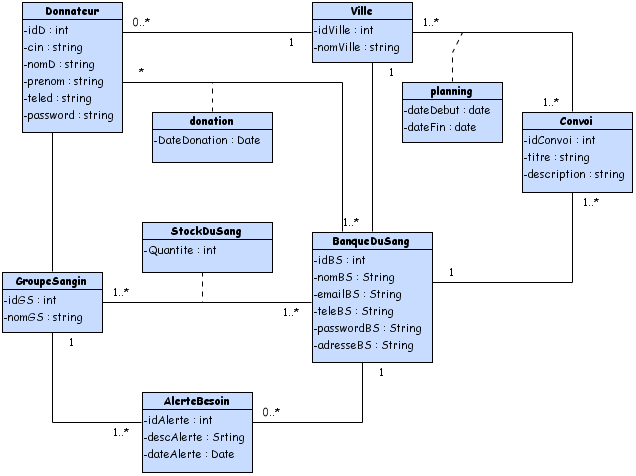
\includegraphics[width=15cm]{Images/chapitre3/class.png}
					 \centering
					 \caption{\label{classe} Diagramme de classe}
				\end{figure}
		}
	}
	
	\newpage
	
	\chapter{Etude technique \& Réalisation}{
		Après avoir exprimé les différentes fonctionnalités envisagées par l’application, ainsi que sa conception, On va présenter dans ce chapitre l’architecture technique du projet et les outils et Framework de développement, ainsi que la réalisation informatique de ses composantes. Il s’agit de la mise en oeuvre des principales fonctions proposées pour tester le fonctionnement du l’application.
	\newpage
	}
	\section{Choix des outils \& technologies :}{
	}
	\section{Présentation de l'application :}{
	}
	\chapter*{Conclusion \& Percpectives}
	\addcontentsline{toc}{chapter}{Conclusion \& Percpectives}
	\markboth{CONCLUSION \& PERCPECTIVES}{CONCLUSION \& PERCPECTIVES}
	\label{chap:conclusion}{
		Ce rapport présente brièvement le projet que j'étais amené à réaliser dans la période de mon stage. Pour mettre en oeuvre ce projet j'ai établi dans un premier lieu
une étude de l'existant et une analyse des diffrents besoins suivie par une étude conceptuelle du sujet affin de dégager les différents fonctionnalités du système ainsi qu'une étude des outils et technologies qui seront utilisés pour la réalisation de l'application.

j'ai essayé au maximum de respecter les fonctionnalités exigées par le cahier de charge.

Sur le plan personnel, ce stage était pour moi une opportunité et une expérience très satisfaisante et enrichissante, grâce à ce stage j'ai appris et j'ai approfondis des connaissances sur des nouvelles technologies, j'ai eu la chance de découvrir le monde du web en temps réel qui est de plus en plus présent dans l'informatique.

Comme perspectives de ce travail, j'ai voulu ajouter des nouvelles fonctionnalités comme l’échange des messages entre les différentes entité du système, et j'ai voulu aussi entamer une partie très importante qui est la partie des tests (Il s'agit d'un effort personnel et non demandé), j'ai commencé quelques tests, mais suite à des contraintes de temps, j'ai pas pu les terminer.

En somme ce stage m'a permis de mettre en pratique et d'approfondir les connaissances reçues au cours de ma première année à l'École nationale supérieure d'informatique et d'analyse des systèmes. Ce stage s'est très bien déroulé, et a été pour moi une véritable opportunité d'apprendre, de découvrir et d'être plus efficace.
	}

\renewcommand{\bibname}{Bibliographie et Webographie}
\begin{thebibliography}{3}
	\bibliographystyle{alpha}
	\addcontentsline{toc}{chapter}{Bibliographie et Webographie}

	\bibitem{valScrum}[En ligne] Disponible sur :
	\\\texttt{http ://blog. Dcube.fr/index.php/2014/04/28/scrum-vs-cycle-en-v-2-2/}

	\bibitem{roleScrum}[En ligne] Disponible sur :
	\\\texttt{http ://blog. Dcube.fr/index.php/2014/04/28/scrum-vs-cycle-en-v-2-2/}

	\bibitem{backlog}[En ligne] Disponible sur :
	\\\texttt{http ://blog. Dcube.fr/index.php/2014/04/28/scrum-vs-cycle-en-v-2-2/}

	\bibitem{jee}[En ligne] Disponible sur :
	\\\texttt{https://docs.oracle.com/javaee/}

	\bibitem{spring}[En ligne] Disponible sur :
	\\\texttt{https://github.com/spring-projects/spring-framework}

	\bibitem{intellij}[En ligne] Disponible sur :
	\\\texttt{https://fr.wikipedia.org/wiki/IntelliJ\_IDEA}

	\bibitem{boot}[En ligne] Disponible sur :
	\\\texttt{http://www.neo-soft-solutions.fr/spring-boot-kesako/}

	\bibitem{rest}[En ligne] Disponible sur :
	\\\texttt{https://fr.wikipedia.org/wiki/Representational\_state\_transfer}

	\bibitem{angular}[En ligne] Disponible sur :
	\\\texttt{https://fr.wikipedia.org/wiki/Angular}

	\bibitem{hibernate}[En ligne] Disponible sur :
	\\\texttt{https://www.jmdoudoux.fr/java/dej/chap-hibernate.htm}

	\bibitem{mysql}[En ligne] Disponible sur :
	\\\texttt{https://fr.wikipedia.org/wiki/MySQL}

	\bibitem{mongo}[En ligne] Disponible sur :
	\\\texttt{https://www.ideematic.com/dictionnaire-digital/mongodb/}

	\bibitem{maven}[En ligne] Disponible sur :
	\\\texttt{https://fr.wikipedia.org/wiki/Apache\_Maven}

	\bibitem{npm}[En ligne] Disponible sur :
	\\\texttt{https://fr.wikipedia.org/wiki/Npm}

	\bibitem{git}[En ligne] Disponible sur :
	\\\texttt{https://fr.wikipedia.org/wiki/Git}

	\bibitem{github}[En ligne] Disponible sur :
	\\\texttt{https://fr.wikipedia.org/wiki/GitHub}
\end{thebibliography}
\end{document}
